\documentclass[12pt,compress,aspectratio=169,dvipsnames]{beamer}
\usetheme{metropolis}
\setbeamersize{text margin left=.5cm,text margin right=.5cm}
\usepackage[lf]{carlito}
\usepackage{siunitx}
\usepackage{tikz}
\usepackage{mathpazo}
\usepackage{bm}
\usepackage{mathtools}
\usepackage[ISO]{diffcoeff}
\diffdef{}{ op-symbol=\mathsf{d} }
\usepackage{xcolor,colortbl}

  
\title{Relative Motion}
\author[TML]{Dr.\ Timothy Leung}
\institute{Olympiads School}
\date{Updated: Summer 2022}

\newcommand{\pic}[2]{
  \includegraphics[width=#1\textwidth]{#2}
}
\newcommand{\eq}[2]{
  \vspace{#1}{\Large
    \begin{displaymath}
      #2
    \end{displaymath}
  }
}
%\newcommand{\iii}{\ensuremath\hat{\bm{\imath}}}
%\newcommand{\jjj}{\ensuremath\hat{\bm{\jmath}}}
%\newcommand{\kkk}{\ensuremath\hat{\bm{k}}}
%\newcommand{\iii}{\ensuremath\hat x}
%\newcommand{\jjj}{\ensuremath\hat y}
%\newcommand{\kkk}{\ensuremath\hat z}


\begin{document}

\begin{frame}{Relative Motion}
  
  \begin{block}{}
    \textbf{All motion quantities must be measured relative to a
      \emph{frame of reference}}
  \end{block}

  \vspace{.2in}
  \begin{itemize}
  \item\textbf{Frame of reference:} the \emph{coordinate system} from which all
    physical measurements are made.
  \item In \emph{classical} mechanics, the coordinate system is the
    Cartesian system
  \item There is no absolute motion/rest: all motions are relative
  \item\textbf{Principle of Relativity:} All laws of physics are equal in all
    inertial (non-accelerating) frames of reference
  \end{itemize}
\end{frame}  



\begin{frame}{Relative Motion}
  \begin{columns}
    \column{.45\textwidth}
    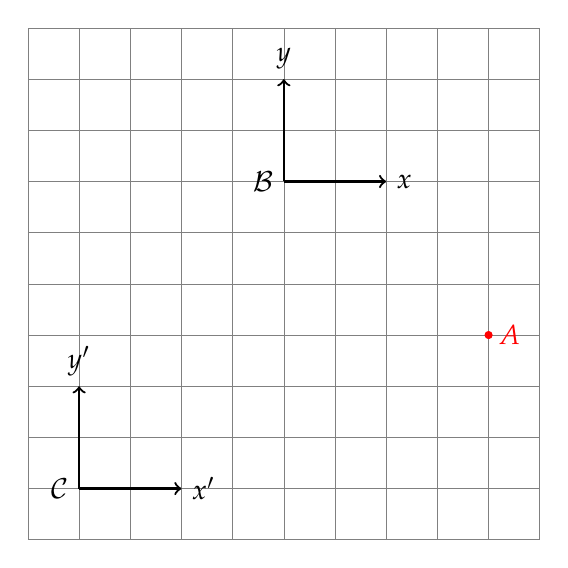
\begin{tikzpicture}[scale=1.3]
      \draw[help lines,step=.5](-.5,-.5) grid (4.5,4.5);
      \begin{scope}[->,thick]
        \draw(0,0)--(1,0) node[right]{$x'$} node[pos=0,left]{$\mathcal C$};
        \draw(0,0)--(0,1) node[above]{$y'$};
        \draw(2,3)--(3,3) node[right]{$x$}  node[pos=0,left]{$\mathcal B$};
        \draw(2,3)--(2,4) node[above]{$y$};
      \end{scope}
      \fill[red] (4,1.5) circle(.04) node[right]{$A$};
    \end{tikzpicture}
    
    \column{.55\textwidth}
    Two frames of reference
    \begin{itemize}
    \item $\mathcal B$ with axes $x,y$
    \item $\mathcal C$ with axes $x',y'$
    \end{itemize}
    The two reference frames may (or may not) be moving relative to each other.
    The motion of the two reference frames affect how motion of
    $\color{red} A$ is calculated.
  \end{columns}
\end{frame}


\begin{frame}{Relative Motion}
  \begin{columns}
    \column{.45\textwidth}
    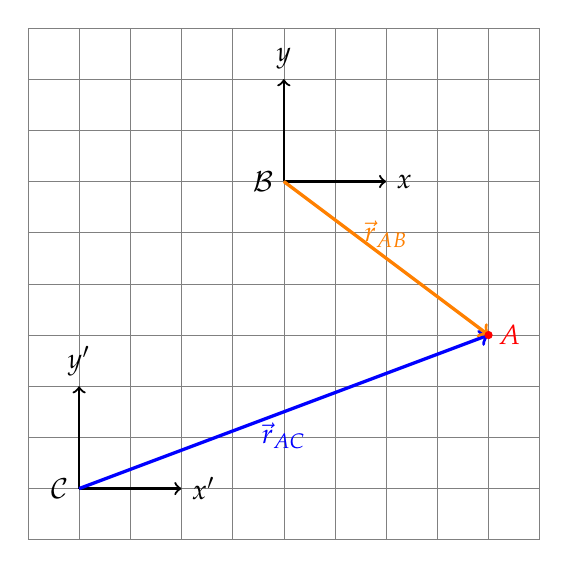
\begin{tikzpicture}[scale=1.3]
      \draw[help lines,step=.5](-.5,-.5) grid (4.5,4.5);
      \begin{scope}[->,thick]
        \draw(0,0)--(1,0) node[right]{$x'$} node[pos=0,left]{$\mathcal C$};
        \draw(0,0)--(0,1) node[above]{$y'$};
        \draw(2,3)--(3,3) node[right]{$x$}  node[pos=0,left]{$\mathcal B$};
        \draw(2,3)--(2,4) node[above]{$y$};
      \end{scope}
      \begin{scope}[->,very thick]
        \draw[blue]  (0,0)--(4,1.5) node[midway,below]{$\vec r_{AC}$};
        \draw[orange](2,3)--(4,1.5) node[midway,above]{$\vec r_{AB}$};
      \end{scope}
      \fill[red] (4,1.5) circle(.04) node[right]{$A$};
    \end{tikzpicture}
    
    \column{.55\textwidth}
    The position of $\color{red} A$ can be described by
    \begin{itemize}
    \item $\color{orange}\vec r_{AB}(t)$ (relative to frame $\mathcal B$)
    \item $\color{blue}\vec r_{AC}(t)$ (relative to frame $\mathcal C$)
    \end{itemize}
    It is obvious that $\color{orange}\vec r_{AB}(t)$ and
    $\color{blue}\vec r_{AC}(t)$ are different vectors
  \end{columns}
\end{frame}



\begin{frame}{Relative Motion}
  \begin{columns}
    \column{.45\textwidth}
    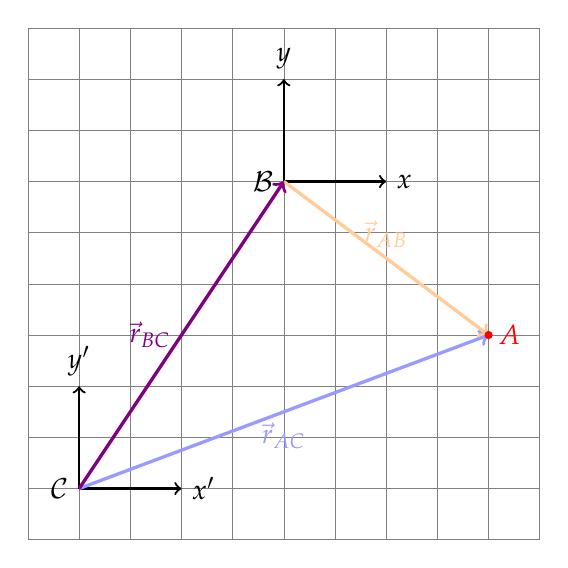
\begin{tikzpicture}[scale=1.3]
      \draw[help lines,step=.5](-.5,-.5) grid (4.5,4.5);
      \begin{scope}[->,thick]
        \draw(0,0)--(1,0) node[right]{$x'$} node[pos=0,left]{$\mathcal C$};
        \draw(0,0)--(0,1) node[above]{$y'$};
        \draw(2,3)--(3,3) node[right]{$x$}  node[pos=0,left]{$\mathcal B$};
        \draw(2,3)--(2,4) node[above]{$y$};
      \end{scope}
      \begin{scope}[->,very thick]
        \draw[blue!40]  (0,0)--(4,1.5) node[midway,below]{$\vec r_{AC}$};
        \draw[orange!40](2,3)--(4,1.5) node[midway,above]{$\vec r_{AB}$};
        \draw[violet](0,0)--(2,3)   node[midway,left] {$\vec r_{BC}$};
      \end{scope}
      \fill[red] (4,1.5) circle(.04) node[right]{$A$};
    \end{tikzpicture}

    \column{.55\textwidth}
%    Starting from the definition of \textbf{relative position}:
%
%    \eq{-.15in}{
%      \boxed{
%        {\color{blue}\vec r_{AC}} =
%        {\color{orange}\vec r_{AB}} + {\color{violet}\vec r_{BC}}
%      }
%    }
%    
%    Differentiating all terms with respect to time, we get the equation for
%    \textbf{relative velocity}:
%
%    \eq{-.15in}{
%      \boxed{
%        {\color{blue}\vec v_{AC}} =
%        {\color{orange}\vec v_{AB}} + {\color{violet}\vec v_{BC}}
%      }
%    }
%
%    Differentiating with respect to time again, and we obtain the expression
%    for \textbf{relative acceleration}:
%
%    \eq{-.15in}{
%      \boxed{
%        {\color{blue}\vec a_{AC}} =
%        {\color{orange}\vec a_{AB}} + {\color{violet}\vec a_{BC}}
%      }
%    }
  \end{columns}
\end{frame}



\begin{frame}{Relative Motion}
  \begin{columns}
    \column{.45\textwidth}
    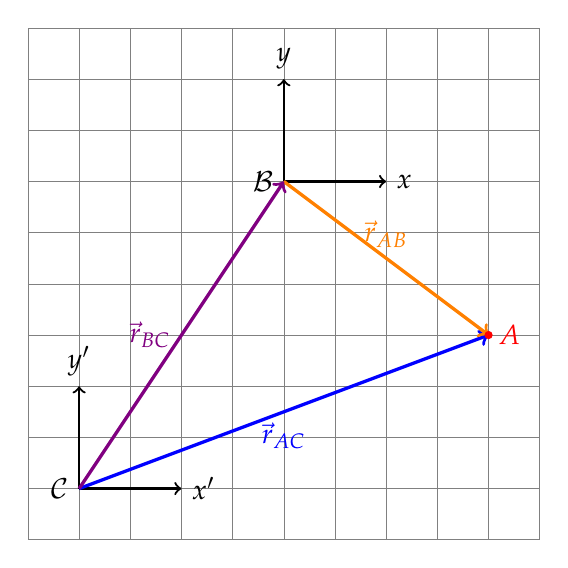
\begin{tikzpicture}[scale=1.3]
      \draw[help lines,step=.5](-.5,-.5) grid (4.5,4.5);
      \begin{scope}[->,thick]
        \draw(0,0)--(1,0) node[right]{$x'$} node[pos=0,left]{$\mathcal C$};
        \draw(0,0)--(0,1) node[above]{$y'$};
        \draw(2,3)--(3,3) node[right]{$x$}  node[pos=0,left]{$\mathcal B$};
        \draw(2,3)--(2,4) node[above]{$y$};
      \end{scope}
      \begin{scope}[->,very thick]
        \draw[blue]  (0,0)--(4,1.5) node[midway,below]{$\vec r_{AC}$};
        \draw[orange](2,3)--(4,1.5) node[midway,above]{$\vec r_{AB}$};
        \draw[violet](0,0)--(2,3)   node[midway,left] {$\vec r_{BC}$};
      \end{scope}
      \fill[red] (4,1.5) circle(.04) node[right]{$A$};
    \end{tikzpicture}

    \column{.55\textwidth}
    Starting from the definition of \textbf{relative position}:

    \eq{-.15in}{
      \boxed{
        {\color{blue}\vec r_{AC}} =
        {\color{orange}\vec r_{AB}} + {\color{violet}\vec r_{BC}}
      }
    }
    
    \vspace{-.2in}Differentiating all terms with respect to time, we get the
    equation for \textbf{relative velocity}:

    \eq{-.15in}{
      \boxed{
        {\color{blue}\vec v_{AC}} =
        {\color{orange}\vec v_{AB}} + {\color{violet}\vec v_{BC}}
      }
    }

    \vspace{-.2in}Differentiating with respect to time again, and we obtain the
    expression for \textbf{relative acceleration}:

    \eq{-.15in}{
      \boxed{
        {\color{blue}\vec a_{AC}} =
        {\color{orange}\vec a_{AB}} + {\color{violet}\vec a_{BC}}
      }
    }
  \end{columns}
\end{frame}



\begin{frame}{Relative Velocity}
  In classical mechanics, the equation for relative velocities follows the
  \textbf{Galilean velocity addition rule}, which applies to speeds much less
  than the speed of light:

  \eq{-.1in}{
    \vec v_{AC}=\vec v_{AB}+\vec v_{BC}
  }

  The velocity of $A$ relative to reference frame $\mathcal C$ is the velocity
  of $A$ relative to reference frame $\mathcal B$, plus the velocity of
  $\mathcal B$ relative to $\mathcal C$. If we add another reference frame
  $\mathcal D$, the equation becomes:

  \eq{-.1in}{
    \vec v_{AD}=\vec v_{AB}+\vec v_{BC}+\vec v_{CD}
  }
\end{frame}
\end{document}
